\section{An interchange format for lexical resources on the Semantic Web: \emph{Lemon}}

\begin{figure}
 \begin{center}

 	 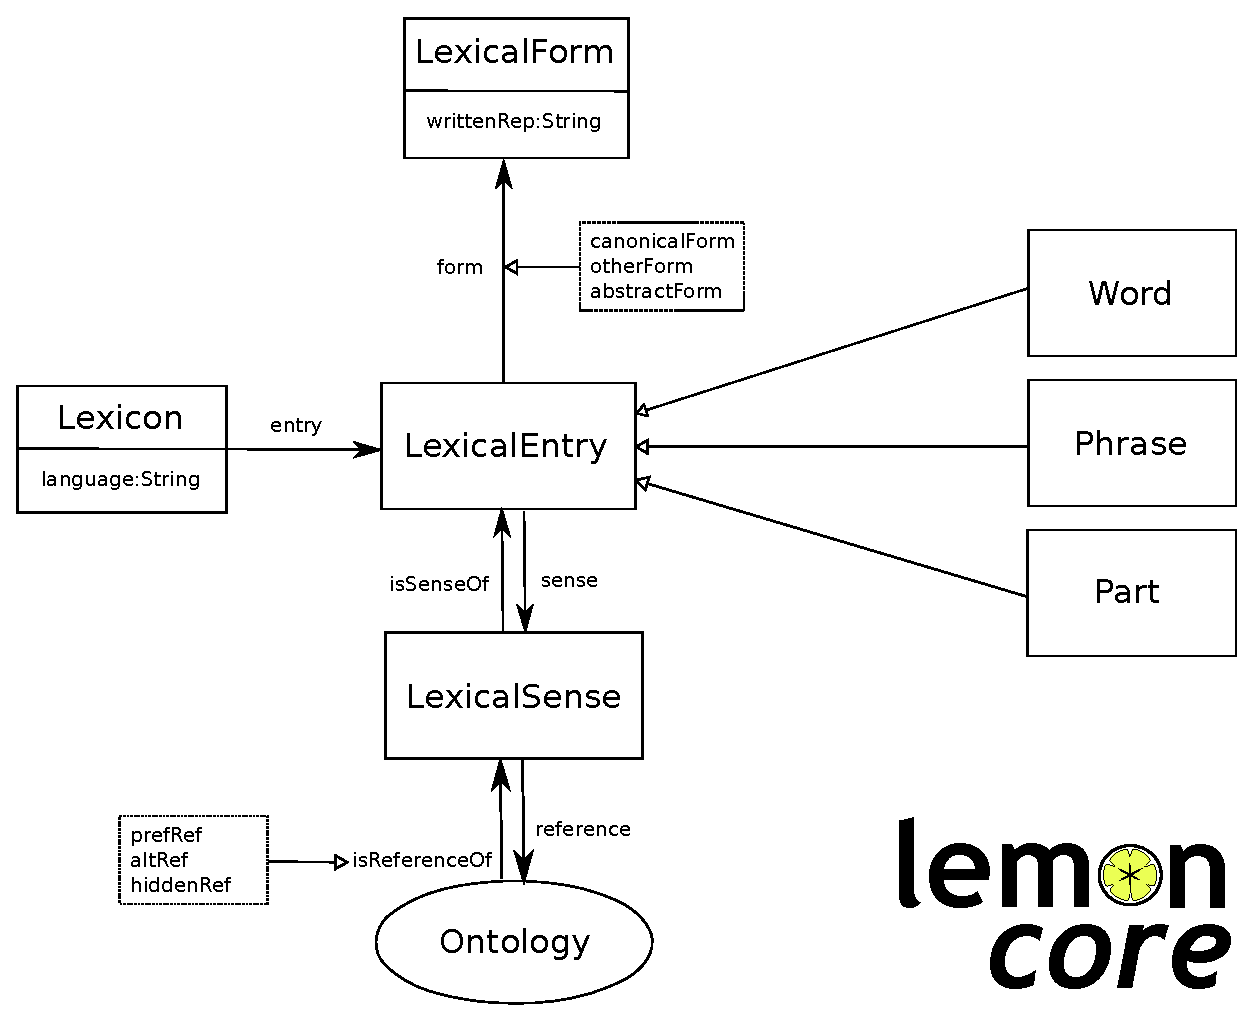
\includegraphics[width=1.0\columnwidth]{images/lemon-core}

 \end{center}
\caption{The core of the \emph{lemon} model\label{lemon-core}}
\end{figure}

\emph{lemon}, a lexicon model for representing and sharing ontology lexica, 
has been proposed as a common interchange format for lexical resources on the Semantic Web\cite{mccrae2012interchanging}. 
Making use of a common interchange format
is important, to integrate resources such as FrameNet and WordNet, which have
been characterised as
complementary resources~\cite{baker2009wordnet}. The RDF version of FrameNet currently available does not adhere to an interchange format such as \emph{lemon}, but is specific to the underlying data model of FrameNet.

%There has been significant work towards integrating lexical resources using RDF and 
%Semantic Web principles~\cite{chiarcos2011towards}, and many resources have already
%been converted to RDF,  notably the conversion of WordNet 
%\cite{van2006conversion}. They provided a simple mapping from WordNet to RDF, and 
%augmented it with OWL semantics so that reasoning could be applied to the structure of the resource.
%However, the format chosen for this resource was specific to the underlying data model of WordNet. 
For this reason, the \emph{lemon} model\cite{mccrae2012interchanging} was proposed  that supports publishing 
lexical-semantic resources as linked data on the basis of the following principles:

\begin{description} 
\item[LMF-based]: To allow easy conversion from non-linked data resources.
\item[RDF-native]: Publishing as linked data, with RDFS and OWL used to describe
  the semantics of the model.
\item[Modular]: Separation of lexicon and ontology layers, so that \emph{lemon} lexica can be linked to existing ontologies
in the linked data cloud.
\item[Externally defined data categories]: Linking to data categories in
  annotation terminology repositories, rather than being limited to a specific part-of-speech tag set.
\item[Principle of least power]: The smaller the model and the less expressive the language, 
	the wider its adoption and the higher the reusability of the
	data\cite{shadbolt2006semantic}.
\end{description}

This core model 
is illustrated in Fig.\ \ref{lemon-core}, which 
defines the
basic elements used by all lexica published as linked data. In addition to this there
are a number of modules used to model linguistic description, syntax, morphology 
and relationships between lexica~\footnote{More detail of the model and descriptions of
the modules can be found at \url{http://lemon-model.net}}.

%\emph{lemon} has been used as a basis for integrating the data of the 
%English Wiktionary, a (human-readable) 
%dictionary created along `wiki' principles, with  
%the RDF version of WordNet \cite{mccrae2012integrating}. \emph{lemon}'s similarity
%to the WordNet model made this conversion straight-forward, with only the need for
%a slight change in modelling to accommodate inflectional variants of lexical
%entries.

